\documentclass[12pt,convert={density=150}]{standalone}

\usepackage{amsmath}
\usepackage{amsfonts}
\usepackage{amssymb}
\usepackage{fontspec}
\usepackage{tikz}

\usetikzlibrary{arrows}
\usetikzlibrary{matrix}
\usetikzlibrary{decorations.markings}

\definecolor{myblue}{RGB}{38,120,179}

\begin{document}
\small
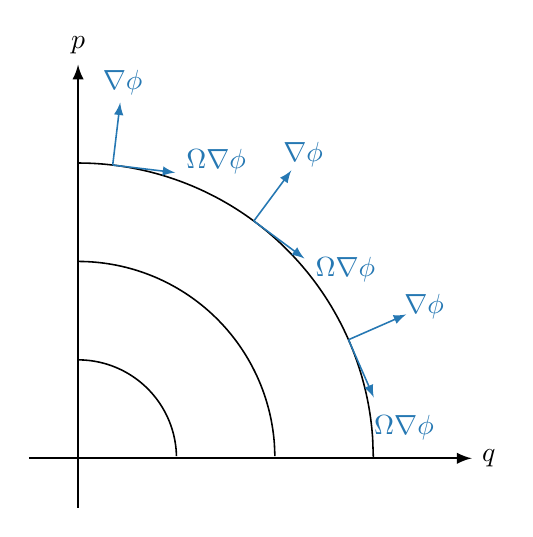
\begin{tikzpicture}[yscale=1.25, xscale=1.25,
    decoration={
        markings,
        mark={
            between positions 0.075 and 0.85 step 1.95cm
            with {	\draw[myblue, -latex] (0,0mm) -- (0,8mm);
		            \draw[myblue] (0,10.5mm) node {$\nabla \phi$};
            		\draw[myblue, -latex] (0,0mm) -- (8mm,0);
		            \draw[myblue] (13mm,2mm) node {$\Omega \nabla \phi$};
		         }
        }}
    ]
      \draw[-latex, line width=0.3mm] (-.5,0) -- (4,0) node[right] {$q$};
      \draw[-latex, line width=0.3mm] (0,-.5) -- (0,4) node[above] {$p$};
      \draw[black, line width=0.2mm, domain=0:3, samples=422, postaction=decorate] plot ({\x},{sqrt(9-\x^2)});
      \draw[black, line width=0.2mm, domain=0:2, samples=381] plot ({\x},{sqrt(4-\x^2)});
      \draw[black, line width=0.2mm, domain=0:1, samples=421] plot ({\x},{sqrt(1-\x^2)});
%      \draw[domain=0:3.015, black, postaction=decorate] plot ({\x},{4*sqrt(cos(deg(\x/2)))-1});
%      \draw[domain=0:2.190, black] plot ({\x},{3*sqrt(cos(deg(\x/1.5)))-1});
%      \draw[domain=0:1.320, black] plot ({\x},{2*sqrt(cos(deg(\x)))-1});
    \end{tikzpicture}
\end{document}

